\documentclass{article}
\usepackage[utf8]{inputenc}
\usepackage{geometry}
\usepackage{graphicx}
\usepackage[hidelinks]{hyperref}

% \title{Habits of a Successful Project Manager}
% \author{Shashank Verma \\ 40217257
% \\
% \\
% \\
% SOEN 6841: Software Project Management}
% \date{30/10/2023}


\begin{document}

% \maketitle
\begin{titlepage}
    \centering
    \vspace*{1cm}
    
\includegraphics[width=0.6\textwidth]{Logo.jpg} % Replace with your university logo
    \par\vspace{0.5cm}
    {\Huge\textbf{Habits of a Successful Project Manager}\par}
    \vspace{1.5cm}
    {\Large\textbf{Shashank Verma}\par}
    \vspace{0.5cm}
    {Student ID: 40217257\par}
    \vspace{2cm}
    {\Large\textbf{SOEN 6841: Software Project Management}\par}
    \vspace{1cm}
    {\large\textbf{Submitted to Professor Pankaj Kamthan}\par} % Replace with your professor's name
    \vfill
    {\large\textbf{Date: 30/10/2023}\par}
\end{titlepage}
\pagenumbering{gobble}

\newpage
\tableofcontents
\newpage
\pagenumbering{arabic}

\addcontentsline{toc}{section}{Abstract}
\section*{Abstract}
This report presents a thorough analysis of the essential traits and practices characteristic of effective project managers, blending traditional management strategies with the principles outlined in the Scout Law. It emphasizes the significance of combining technical expertise with interpersonal skills to achieve superior project outcomes. The analysis draws from diverse sources, including academic literature, real-world anecdotes from project management workshops, and the author's extensive professional experiences. The crux of this study is the indispensable role of interpersonal skills, alongside a proactive approach to problem-solving and fostering robust workplace relationships. The primary aim is to construct an all-encompassing framework that transcends industry-specific boundaries, thereby improving leadership efficacy and project success rates. By integrating technical acumen with essential soft skills, the report underscores the pivotal influence of human factors in project management. This comprehensive synthesis aspires to bridge the prevailing gap between technical mastery and the nuanced art of human interaction, highlighting their collective importance in the realm of effective project leadership.
\\ \\
\textbf{Keywords}: Project Managers, Scouts Law, Interpersonal Skills, Leadership efficacy, Problem Solving, Soft Skills

\newpage

\section{Introduction}
\subsection{Motivation}
In today's global economy, project managers are widely recognized as essential for project success across various businesses. Their strong management abilities are key to enhancing project productivity and efficiency, complementing advancements in project management tools and processes. The human element, represented by project managers' behaviors, remains crucial. Project management now encompasses human dynamics, teamwork, and interpersonal communication alongside technical execution, reflecting the growing demand for project management expertise as organizations adopt project centric approaches. Educational institutions, especially universities, must adapt by offering comprehensive project management courses that proactively prepare future project managers for the evolving work environment, emphasizing a balance between technical and interpersonal skills \cite{pant2008project}. This shift is imperative to meet the changing demands of the business landscape, emphasizing the need for a paradigm change in project management education and perception.

\subsection{Problem Statement}
The primary issue with present project management is the overemphasis on technical abilities, which frequently ignores soft or people skills. Frameworks such as the PMBOK Guide, which emphasise technical skills over soft skills runs the danger of ignoring soft skills that are just as important—like team dynamics, leadership, and communication—also exhibit this mismatch. This argues for a more integrated approach to project management education, emphasising both technical and interpersonal abilities equally. The objective is to produce managers who excel in both the technical and human aspects of project management by matching academic training with industrial needs. This well-rounded approach is essential for producing project managers who can successfully lead projects in the diverse and changing professional environment of today \cite{pant2008project}. 



\subsection{Objectives}
This case study aims to identify the non-technical capabilities that are essential to project managers' success. By doing this, we seek to enhance project leadership development and training within organisations. By emphasising the significance of soft skills in achieving project success, this study offers practitioners and their teams practical insights that can be utilised to improve project managers' abilities.

\section{Background Material}
\subsection{The Scout Law as a Leadership Model}

Effective leadership styles in project management significantly impact a Project Manager's success. Project Managers must not only coordinate tasks but also inspire and guide their teams. Unfortunately, education and training for Project Managers often prioritize technical skills over leadership development. Studies on scouting reveal the importance of a balanced leadership approach. Scouting's focus on individual growth within teams aligns with the requirements for a Project Manager, including adaptability, decision-making, problem-solving, and ethical judgment \cite{kaluzny2022scouting}. Scouting's emphasis on real-world challenges and teamwork closely parallels the needs of Project Managers. Insights from scouting studies show how young individuals develop strategic thinking, communication, and ethical leadership—critical competencies for Project Managers. Combining technical expertise with leadership skills fosters a collaborative environment vital for achieving collective project goals. Education and training for Project Managers must evolve to incorporate these leadership aspects, drawing from scouting methodologies to better prepare future professionals for Project Manager success.

\subsection{Adaptability in the Face of Disruption}

\begin{figure}[htp]
    \centering
    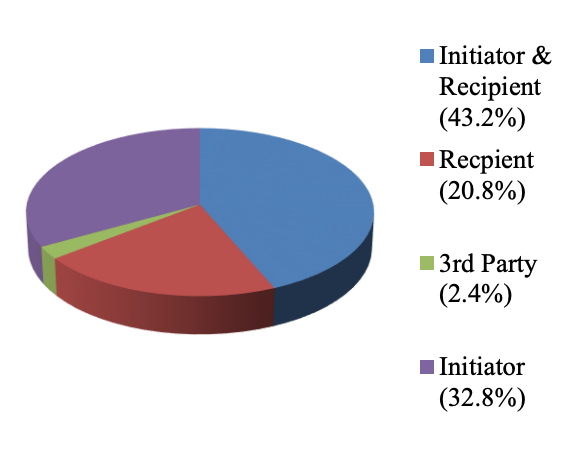
\includegraphics[width=5cm]{Beneficiaries of Interruption.png}
    \caption{Beneficiaries of Interruption \cite{mordu2016managing}}
    \label{fig:Beneficiaries of Interruption}
\end{figure}

In the world of successful Project Management, a Project Manager's ability to effectively manage and adapt to interruptions is crucial. Several studies in the field of engineering consultancy offer examples of how a skilled Project Manager navigated a work environment filled with interruptions, ranging from sudden phone calls to scheduled meetings. Interestingly, these studies found that 43.2\% of these interruptions proved beneficial, contributing to goal achievement and enhancing job satisfaction \cite{mordu2016managing}. This underscores a key trait in effective Project Management: the skill of transforming potential disruptions into opportunities.

In the broader context of Project Management success, exceptional Project Managers excel in assessing the urgency of interruptions and seamlessly integrating them into their workflow without derailing project goals. This ability becomes especially critical in fast-paced work environments where multitasking and adaptability are essential for success.

\subsection{Interpersonal Skills and Organizational Culture in Project Management}

Effective Project Managers rely on their interpersonal skills, including empathy, teamwork, and communication, to build trust with their teams and manage various stakeholders. The organization's culture, whether it promotes collaboration or individualism, significantly influences team dynamics and employee performance \cite{nusari2018impact}.

For a Project Manager, the ability to navigate and balance interpersonal relationships within the prevailing organizational culture is vital. Creating an environment that fosters teamwork and outstanding performance is key to project success. In essence, the Project Manager's skill in harmonizing relationships within the organization's culture directly impacts project outcomes.


\section{Methods \& Methodology}

\subsection{Methodological Framework for Investigating Project Manager Habits}

\subsubsection{Literature Review}

An comprehensive literature analysis was performed using Google Scholar to investigate the habits of successful project managers. The study focused on terms such as "project manager traits," "successful project management habits," and "leadership in project management." The selection criteria was based on publications' relevance, and recentness. A few important studies were "What is a good project manager?" \cite{bredillet2015good}, "Leadership competency profiles of successful project managers" emphasise critical thinking and emotional intelligence \cite{muller2010leadership}; "Patterns in the project managers’ rhythms, habits, routines and rituals" explore daily routines and habits \cite{sigurdhssonpatterns}; and "Project managers’ and change managers’ contribution to success", analyses the roles of project and change management in project success \cite{pollack2016project}. These resources provide an overall perspective on the good habits of a project manager.

\subsubsection{Identification of Key Traits and Practices} 

The key traits and practices of successful project managers identified from the literature review align well with the attributes in the original case study. These include competence in both attribute and performance based dimensions, emphasizing intellectual, managerial, and emotional competencies like critical thinking and emotional intelligence \cite{muller2010leadership}. The importance of organization, communication, and continuous improvement in daily routines \cite{sigurdhssonpatterns}, along with skills in managing costs and navigating organizational change, echoes the workshop's findings on traits like sociability, respectfulness, positive demeanor, and the ability to 'speak truth to power' \cite{bredillet2015good}. This synthesis of literature underscores the consistent themes in defining effective project management practices.

\subsubsection{Inclusion of Diverse Perspectives}

In addressing the problem of identifying successful project management habits, the approach included seeking diverse perspectives from various industries, organizational sizes, and cultural contexts. This was achieved through the analysis of the provided case studies. Each study brought a unique angle: one examined the philosophical underpinnings of what constitutes competence in project management \cite{bredillet2015good}, another focused on leadership competencies in different types of projects \cite{muller2010leadership}, while a third explored the daily habits and routines of project managers \cite{sigurdhssonpatterns}. Additionally, the relationship between project management and change management was considered, highlighting the adaptability of project management practices across different organizational changes \cite{pollack2016project}. This multifaceted approach ensured a comprehensive understanding of project management habits, encompassing a wide range of scenarios and challenges faced in different environments and cultures.

\subsection{Analytical Methods in Deciphering Project Management Traits}

\subsubsection{Thematic Analysis}

The procedure involved systematically using a qualitative analysis approach to classify and identify recurring themes and patterns linked to effective project management practices. By categorizing key characteristics, behaviors, and competencies, the analysis uncovered reoccurring themes. These themes, reflecting the diversity of project management roles across various industries and organizational sizes, included critical thinking, emotional intelligence, effective communication, and adaptability. This approach enabled a deeper insight into the essential routines and habits that are crucial for success in project management, as corroborated by numerous studies.


\subsubsection{Comparative Analysis}

In analyzing the results, a comparative approach was used to discern how factors like project size, industry, or manager experience level influence project management habits. The analysis revealed variations in competencies across project types, showing the impact of industry and complexity \cite{muller2010leadership}. It also highlighted how managerial experience affects the adoption of certain habits \cite{sigurdhssonpatterns} and how organizational context shapes project management approaches, particularly in the interplay between project and change management \cite{pollack2016project}. This method offered a deeper understanding of the varied influences on effective project management practices.

\subsubsection{Synthesis of Findings}

The synthesis of various case studies highlights the multifaceted nature of successful project management, emphasizing the integration of intellectual and emotional competencies with strong ethical considerations \cite{bredillet2015good}. Critical thinking, influence, and motivation are key attributes \cite{muller2010leadership}. Daily habits like effective organization and continuous improvement align with these competencies, demonstrating their practical application in everyday project management \cite{sigurdhssonpatterns}. Additionally, the interaction between project management and change management underscores the need for project managers to navigate organizational changes adeptly, with competencies complementing each role in effective project execution \cite{pollack2016project}. This synthesis reconciles differing perspectives on the balance between soft skills and technical expertise and consistently identifies communication, leadership, and adaptability as central to project managers' effectiveness.

\section{Results Obtained}
\subsection{Conditions}


Effective Project Managers adapt their approaches, balancing ethical and practical competencies that encompass both duty and outcome-focused strategies \cite{bredillet2015good}. In complex projects, this equilibrium blends practical action and wisdom. Leadership skills like strategic vision, adaptability, and effective communication are crucial in larger organizations, while smaller projects prioritize hands-on involvement and personalized leadership styles for an intimate and responsive atmosphere \cite{sigurdhssonpatterns}. Organizational structure, whether matrix or projectized, impacts Project Manager traits, with resource negotiation, conflict management, and cross-functional team leadership being vital in such environments. The project's life cycle stage plays a role, with early stages focusing on planning and risk assessment, and later stages on quality control, team morale, and stakeholder satisfaction. Successful Project Management requires adaptability, tailoring tactics and routines to each project environment \cite{hyvari2006success}.

\subsection{Constraints}

Effective Project Managers recognize that the success of project management traits and methodologies varies based on each project's unique context \cite{muller2010leadership}. Leadership competencies, for instance, depend on factors such as project complexity, strategic importance, and contract type, suggesting that certain leadership traits may not apply universally \cite{sigurdhssonpatterns}. Adaptability is essential in project management, with the capability to modify management styles according to specific project needs \cite{markopoulos2005project}. This adaptability is especially crucial in fast-evolving business environments where external factors like market dynamics and technological advancements can significantly influence project outcomes. Awareness of organizational structure and culture is key, as they influence the efficacy of management techniques. The dynamic and diverse nature of projects requires an adaptive approach, where a manager's success often depends on their ability to adjust to evolving project contexts \cite{pollack2016project}.

\subsection{Quality}

\begin{figure}[htp]
    \centering
    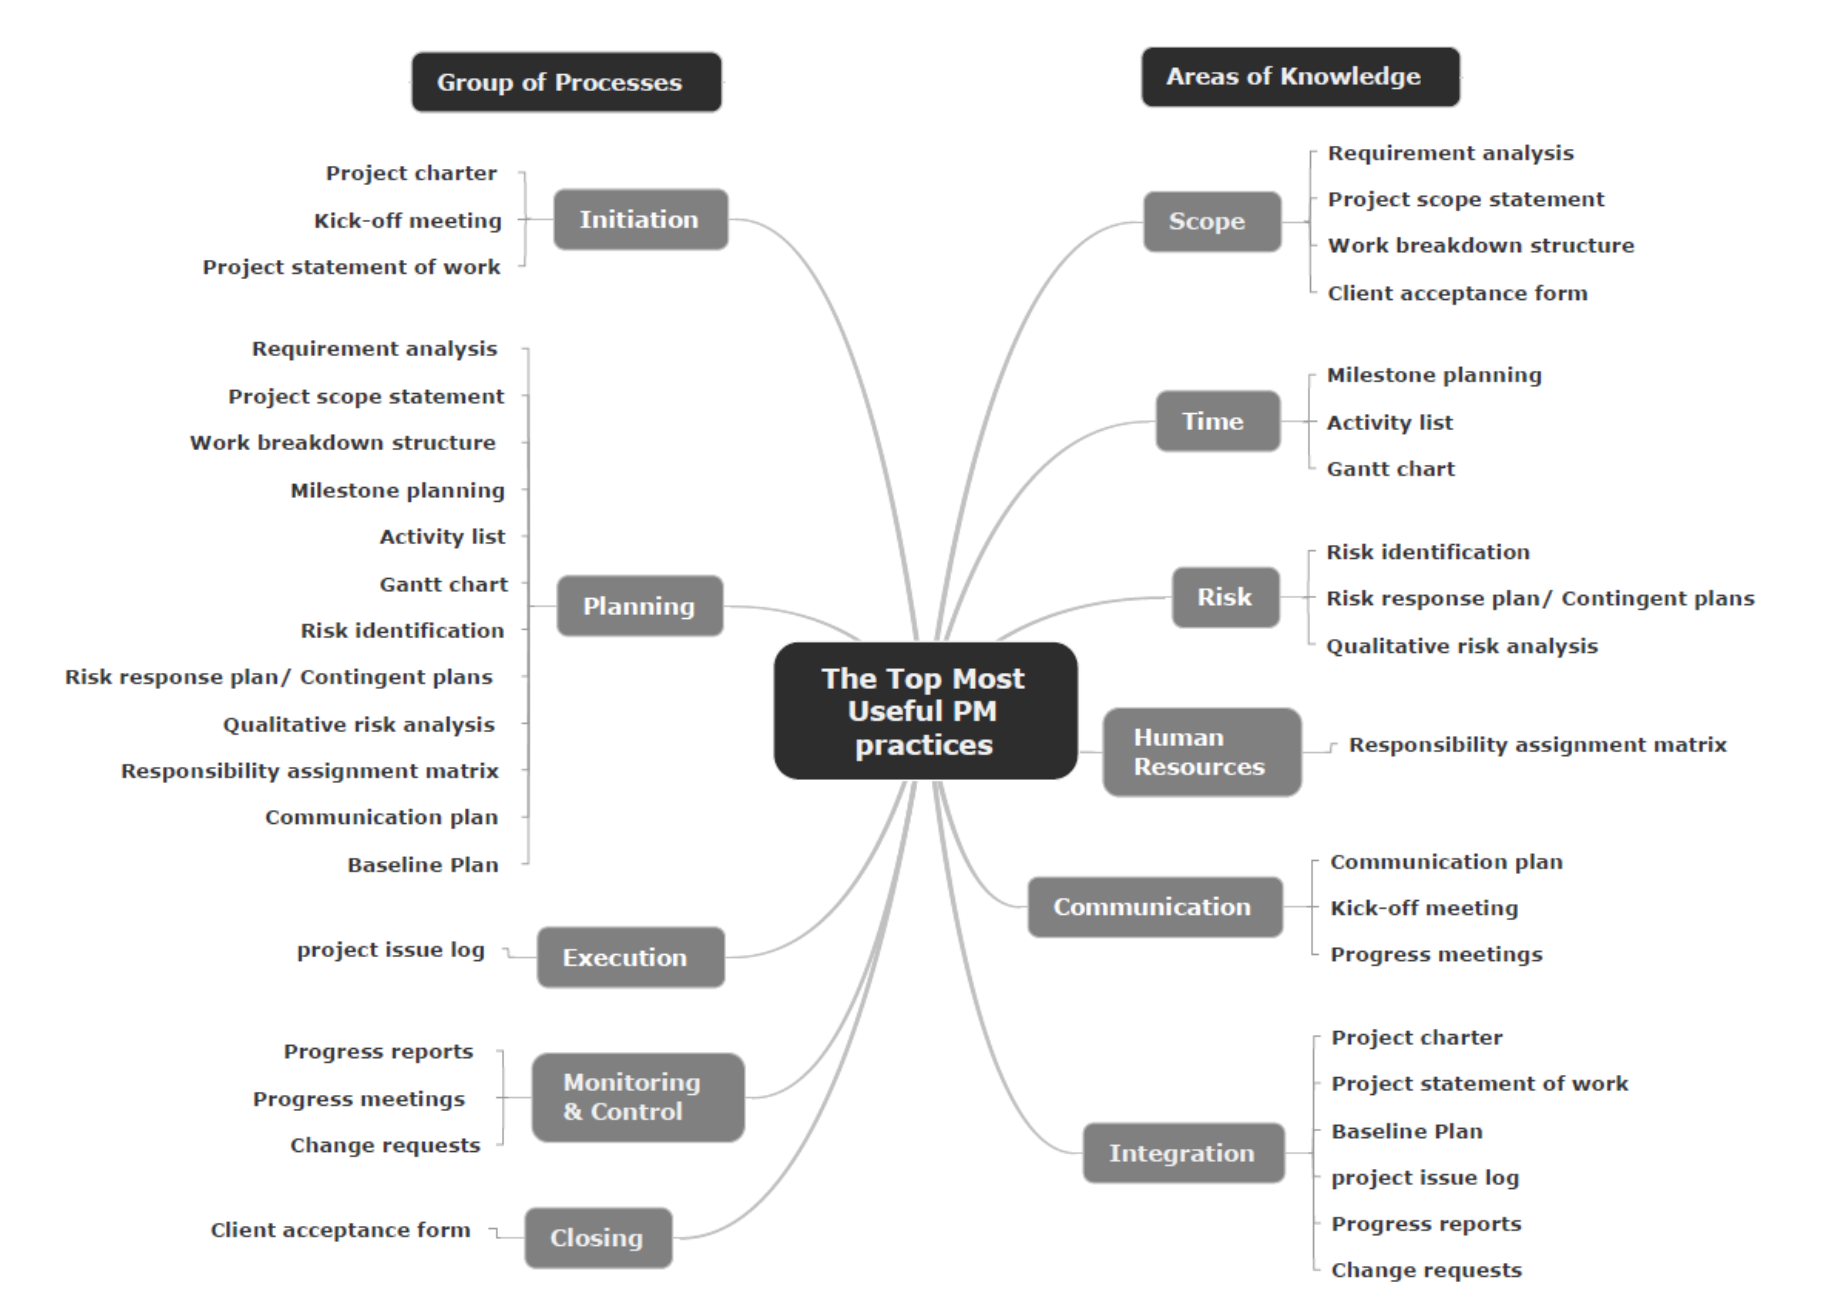
\includegraphics[width=8cm]{Project Manager Practices.png}
    \caption{Project Manager Practices}
    \label{fig:Project Manager Practices}
\end{figure}

Successful project outcomes in project management are closely tied to specific traits and methodologies, as supported by the analysis of 250 large software projects and broader project management practices \cite{jones2004software}. Key contributing traits include robust project planning, accurate cost estimating, effective milestone tracking, stringent change control, and rigorous quality control. These qualities are evident in successful projects and are crucial for handling complexities like changing requirements and defect removal efficiency, whereas projects facing overruns or cancellation often lack them, with poor quality control being a primary contributor to failures. Additionally, stakeholder engagement, risk management, strategic planning, and effective communication are vital across various project types and contexts \cite{fernandes2013identifying}. These practices significantly impact success metrics such as budget adherence, stakeholder satisfaction, and timely completion. Strategic planning helps navigate challenging project landscapes, effective communication ensures alignment with project objectives, stakeholder engagement maintains support and satisfaction, and risk management identifies and addresses potential issues. These insights highlight the necessity of thorough planning, stakeholder management, and quality control in achieving successful project outcomes in effective project management.

\section{Critical Thinking}

\subsection{Critical Analysis}

The qualities that have been emphasized—such as leadership, flexibility, and people skills—have an intrinsic value but may not be applicable in every situation. The importance of closely evaluating these attributes' effectiveness in a range of project situations is highlighted by their focus. For instance, leadership philosophies that work well in one organisational or cultural setting might not work well in another. Moreover, even if there is evidence linking management attributes to project performance, this connection begs concerns regarding the all-encompassing success criteria. Conventional metrics typically concentrate on meeting deadlines and staying within budget, but a more comprehensive assessment should also take into account long-term effects, team happiness, and alignment with larger organisational goals. These subtle factors frequently extend beyond what case studies normally cover.

\subsection{Assessment of Methodology}

The methodology employed relies heavily on literature reviews and case studies, which may introduce potential inaccuracies or biases. It's essential to investigate whether the sources encompass a wider range of industries and project types to ensure a more comprehensive perspective, as an excessive focus on specific areas can result in a skewed viewpoint. Furthermore, while diverse fields were examined, it's worth considering whether they authentically represent the diverse array of cultural and organizational contexts that exist. This assessment plays a vital role in assessing the global applicability of these findings.

\subsection{Future Research}

The existing framework provides a solid foundation for understanding effective project management, but there are opportunities for future investigations. For instance, it would be valuable to examine how these habits adapt and apply to emerging industries. Additionally, considering the growing prevalence of remote or virtual project teams, further research could delve into how these habits manifest in such settings. Expanding the scope of research to encompass various industry sectors, including non-traditional project environments, could yield insights into the applicability of these habits across diverse contexts.

\section{Conclusions and Future Works}
\subsection{Suggested Improvements}

There are several critical areas in the field of project management that warrant further study and development to enhance the efficiency of project managers. First, managing project complexity necessitates the creation of new frameworks and tools. Second, focusing on the social dynamics of project management, including stakeholder engagement, team dynamics, and interpersonal relationships, is essential for project success. Third, aligning project goals with organizational objectives and stakeholder values is crucial for value generation, requiring a better understanding of how to integrate broader company goals into project design and implementation. Additionally, early project conception phases underscore the need for excellent project planning and strategic abilities. Lastly, advancing the skills of project managers is vital, with a growing demand for training that encompasses critical thinking, flexibility, and reflective practices, enabling them to lead and navigate complex and dynamic project environments effectively \cite{winter2006directions}. Collectively, these areas are pivotal for advancing the field of project management, ensuring that managers possess the necessary skills and knowledge to successfully oversee projects in diverse settings.


\subsection{Limitations to Solution}

% Describe scenarions where the solutions dont work well enough

In the field of project management, both organizational limitations and the personal qualities of the project manager significantly influence the effectiveness of common practices and traits. Ineffective leadership characterized by negative personal traits such as poor communication, authority misuse, or inexperience can undermine a project's success, underscoring the importance of interpersonal and leadership abilities alongside technical expertise. Organizational limitations, including resource constraints, inadequate planning, and a lack of support from upper management, can pose significant challenges. These constraints can restrict a project manager's ability to implement best practices and achieve project objectives, highlighting the need for flexibility and adaptation in project management. Project managers must possess a diverse skill set to navigate various obstacles in different project environments and develop techniques that are resilient, flexible, and capable of addressing complex situations while overcoming individual and institutional constraints \cite{toor2009ineffective}.

\subsection{Applications in Real World}
% Benefits in real world.
The use of methodologies like PERT and CPM across industries underscores the significance of adaptability, strategic planning, and data-driven decision-making in project management \cite{cicmil2006rethinking}. These methodologies optimize project duration and cost, emphasizing effective time and resource management in complex projects. Their versatility proves valuable for diverse projects, regardless of scale or type, highlighting the importance of data-driven approaches. In real-world industry projects, as opposed to academic settings, a blend of theoretical knowledge and practical adaptability is essential. Real-world projects demand flexibility, real-time problem-solving, and adaptability to ever-changing stakeholder expectations and project scopes, requiring the practical application of project management principles to navigate complexities \cite{toor2009ineffective}.

\subsection{Conclusion}
% Short summary.

To handle complicated projects, effective project management requires an all-encompassing and flexible strategy that integrates cutting-edge approaches and tools. With an emphasis on the social dimensions of project management, it's vital to match organisational goals with project goals and develop managers' critical thinking and adaptability skills. Project managers must possess a variety of skills and flexibility in order to efficiently traverse different project contexts and overcome personal and organisational problems. The practical use of techniques such as PERT and CPM highlights the significance of strategic planning and data-informed decision-making. At the end of the day, effective project management is about combining academic understanding with real-world flexibility, which means that ongoing education and development are required to stay up with the ever-changing project environment.



% \section{References}


% \subsection{Appendix}
% external references here

% \subsection{Acknowledgements}
% ACKS

\bibliographystyle{IEEEtran}
\addcontentsline{toc}{section}{References}
\bibliography{references}

\end{document}
